% author: Ondrej Platek 2012
%settings are located in begin_settins.tex and end_settings.tex files
%do not remove!
%% Verze pro jednostranný tisk:
% Okraje: levý 40mm, pravý 25mm, horní a dolní 25mm
% (ale pozor, LaTeX si sám přidává 1in)
%\documentclass[12pt,a4paper]{report}
%\setlength\textwidth{145mm}
%\setlength\textheight{247mm}
%\setlength\oddsidemargin{15mm}
%\setlength\evensidemargin{15mm}
%\setlength\topmargin{0mm}
%\setlength\headsep{0mm}
%\setlength\headheight{0mm}
% \openright zařídí, aby následující text začínal na pravé straně knihy
%\let\openright=\clearpage

%% Pokud tiskneme oboustranně:
\documentclass[12pt,a4paper,twoside,openright]{report}
\setlength\textwidth{145mm}
\setlength\textheight{247mm}
\setlength\oddsidemargin{15mm}
\setlength\evensidemargin{0mm}
\setlength\topmargin{0mm}
\setlength\headsep{0mm}
\setlength\headheight{0mm}
\let\openright=\cleardoublepage

%% Pokud používáte csLaTeX (doporučeno):
%\usepackage{czech}
%% Pokud nikoliv:
%\usepackage[czech]{babel}
% \usepackage[T1]{fontenc}

%%%% ENCODING: usually latin2, cp1250 nebo utf8 %%%
\usepackage[utf8x]{inputenc}

%%%%% OTHER PACKAGES  %%%%%
% \usepackage{doxygen} % wrong sty! 
\usepackage{pdfpages}
\usepackage{listings}
\usepackage{color}
\usepackage{graphicx}
\usepackage{amsthm}


\usepackage{draftwatermark} 
\SetWatermarkScale{4}
\SetWatermarkLightness{0.5}
\SetWatermarkText{Draft!}

\usepackage{multirow} 
\usepackage[table]{xcolor}

\usepackage{amsmath, amsthm, amssymb}
\usepackage[round]{natbib} % citace

%% Balíček hyperref, kterým jdou vyrábět klikací odkazy v PDF,
%% ale hlavně ho používáme k uložení metadat do PDF (včetně obsahu).
%\usepackage[ps2pdf,unicode]{hyperref}   % Musí být za všemi ostatními balíčky
\usepackage[unicode]{hyperref}   % Musí být za všemi ostatními balíčky
\hypersetup{pdftitle=Diploma thesis}   % TODO check if correct
% \hypersetup{pdfauthor=Ondřej Plátek}
\hypersetup{pdfauthor=Ondrej Platek}


%%% MACROS %%%% 
% Tato makra přesvědčují mírně ošklivým trikem LaTeX, aby hlavičky kapitol
% sázel příčetněji a nevynechával nad nimi spoustu místa. Směle ignorujte.
\makeatletter
\def\@makechapterhead#1{
  {\parindent \z@ \raggedright \normalfont
   \Huge\bfseries \thechapter. #1
   \par\nobreak
   \vskip 20\p@
}}
\def\@makeschapterhead#1{
  {\parindent \z@ \raggedright \normalfont
   \Huge\bfseries #1
   \par\nobreak
   \vskip 20\p@
}}
\makeatother

% Toto makro definuje kapitolu, která není očíslovaná, ale je uvedena v obsahu.
\def\chapwithtoc#1{
\chapter*{#1}
\addcontentsline{toc}{chapter}{#1}
}

%%% TODO makra
\def\todo#1{
\emph{\color{red} TODO: #1}
}

\def\todon#1{
  \todo{#1 \\}
}
% references to footnote
% usage: \footnoteremember{myfootnote}{This is my footnote} and then \footnoterecall{myfootnote} 
\newcommand{\footnoteremember}[2]{
    \footnote{#2}
    \newcounter{#1}
    \setcounter{#1}{\value{footnote}}
}
\newcommand{\footnoterecall}[1]{
    \footnotemark[\value{#1}]
}
\graphicspath{{./images/}}

% includes file with code
% usage: \code{MyCodeName}{../testapp/models.py}
\newcommand{\code}[3]{
  \hrulefill
  \subsubsection*{#1}
  \lstinputlisting[style=#2]{#3}
  \vspace{2em}
}


%%% END OF MACROS %%%
\begin{document}


../text/snippets/python_style.tex % do not remove

\maketitle
% \note[item]{Good afternoon, ... DO NOT READ IT, POINT AT IT!}


\begin{frame}\frametitle{TODOS} 
    \begin{itemize}
        \item write intro
        \item print the slides and write my talk
        \item practise it
        \item add link to the README to this slides
        \item picture of real lattice from my blog
    \end{itemize}
\end{frame}


\begin{frame} \frametitle{Content} \tableofcontents \end{frame}


\section{Motivation} %%%%%%%%%%%%%%%%%%%%%%%%%%%%%%%%%%%%%%%%%%%%%%%%%%%%%%%%

\begin{frame}\frametitle{Problem} 
    Spoken dialogue systems needs speech recognition \\
    OpenJulius --- crashes, PocketSphinx --- no posteriors, RWTH decoder --- license \\
    Cloud based services Google and Nuance --- no customisation + license issues
\end{frame}

\begin{frame}\frametitle{Goals of thesis} 
Goals of the thesis were:
    \begin{itemize}
        \item to build acoustic models using the Kaldi toolkit,
        \item to develop new real-time recogniser which supports incremental speech recognition,
        \item to integrate the~recogniser into our Alex SDS.
    \end{itemize}
\end{frame}


\section{ASR introduction} %%%%%%%%%%%%%%%%%%%%%%%%%%%%%%%%%%%%%%%%%%%%%%%%%%%%%%%%

\begin{frame}\frametitle{ASR components} 
    % Generated with LaTeXDraw 2.0.8
% Sun Jul 07 00:14:55 CEST 2013
% \usepackage[usenames,dvipsnames]{pstricks}
% \usepackage{epsfig}
% \usepackage{pst-grad} % For gradients
% \usepackage{pst-plot} % For axes
\scalebox{0.8} % Change this value to rescale the drawing.
{
\begin{pspicture}(0,-3.7639062)(9.26,3.7639062)
\usefont{T1}{ptm}{m}{n}
\rput(2.0,3.3){\psovalbox{Speech Input}}
\psline[linewidth=0.04cm,arrowsize=0.05cm 2.0,arrowlength=1.4,arrowinset=0.4]{->}(2.0,2.8)(2.0,2.3)
\usefont{T1}{ptm}{m}{n}
\rput(2.0454688,1.5789063){\psdblframebox[framesep=10pt]{Signal processing}}
\usefont{T1}{ptm}{m}{n}
\rput(2.0,0.3){\psovalbox{Acoustic observations $a$\tiny For example \acs{MFCC}}}
\psline[linewidth=0.04cm,arrowsize=0.05cm 2.0,arrowlength=1.4,arrowinset=0.4]{->}(2.0,0.9)(2.0,0.3)
\usefont{T1}{ptm}{m}{n}
\rput(2.0,-0.9){\psdblframebox[framesep=10pt]{Decoding $w^*$: \small $argmax_{w} P(a \mid w)*P(w)$}}
\usefont{T1}{ptm}{m}{n}
\rput(2.0,-1.6210938){}
\usefont{T1}{ptm}{m}{n}
\rput(8.5,-0.5){\psframebox{Language model: $P(w)$}}
\psline[linewidth=0.04cm,arrowsize=0.05cm 2.0,arrowlength=1.4,arrowinset=0.4]{<-}(5.8,-0.6)(6.3,-0.6)
\rput(8.7,-1.3){\psframebox{Acoustic model: $P(a \mid w)$}}
\psline[linewidth=0.04cm,arrowsize=0.05cm 2.0,arrowlength=1.4,arrowinset=0.4]{<-}(5.8,-1.2)(6.3,-1.2)
\usefont{T1}{ptm}{m}{n}
\rput(2.0, -2.4){\psovalbox{Recognized words $w^*$}}
\psline[linewidth=0.04cm,arrowsize=0.05cm 2.0,arrowlength=1.4,arrowinset=0.4]{->}(2.0,-1.5)(2.0,-1.9)
\end{pspicture} 
}

    % Architecture of statistical speech recognizer\cite{ney1990acoustic}
\end{frame}

\begin{frame}\frametitle{Acoustic features, features preprocessing} 
    % Generated with LaTeXDraw 2.0.8
% Sun Jul 07 00:14:55 CEST 2013
% \usepackage[usenames,dvipsnames]{pstricks}
% \usepackage{epsfig}
% \usepackage{pst-grad} % For gradients
% \usepackage{pst-plot} % For axes
\scalebox{1} % Change this value to rescale the drawing.
{
\begin{pspicture}(9,4)
\usefont{T1}{ptm}{m}{n}

\rput(8.0,3.0){$frames$=7}

\psframe[linecolor=blue, linestyle=dashed, linewidth=0.04,dimen=outer](0.0,1.0)(3.0,2.0)
\psframe[linecolor=black,linestyle=dashed, linewidth=0.04,dimen=outer](1.0,1.1)(4.0,2.1)
\psframe[linecolor=orange,linestyle=dashed, linewidth=0.04,dimen=outer](2.0,1.2)(5.0,2.2)
\psframe[linecolor=green, linestyle=dashed, linewidth=0.04,dimen=outer](3.0,1.3)(6.0,2.3)
\psframe[linecolor=blue,linestyle=dashed, linewidth=0.04,dimen=outer](4.0,1.4)(7.0,2.4)
\psframe[linecolor=black,linestyle=dashed, linewidth=0.04,dimen=outer](5.0,1.5)(8.0,2.5)
\psframe[linecolor=orange, linestyle=dashed, linewidth=0.04,dimen=outer](6.0,1.6)(9.0,2.6)

\rput(1.0,2.9){$shift=10ms$}
\psline[linewidth=0.04cm,arrowsize=0.05cm 2.0,arrowlength=2.0,arrowinset=0.4]{<->}(0.0,2.5)(1.0,2.5)

\rput(7.5,0.9){$win\_len=25ms$}
\psline[linewidth=0.04cm,arrowsize=0.05cm 2.0,arrowlength=2.0,arrowinset=0.4]{<->}(6.0,0.5)(9.0,0.5)

\rput(4.0,0.4){ $audio\_len=85ms$  }
\psline[linewidth=0.04cm,arrowsize=0.05cm 2.0,arrowlength=2.0,arrowinset=0.4]{<->}(0.0,0.0)(9.0,0.0)
\end{pspicture} 
}

    ../../text/images/mfcc-delta.tex
    % \caption{\ac{PLP} or \ac{MFCC} features are computed every 10 ms seconds in 25 ms windows.
    % Audio length is $(frames-1)*shift + win\_len = 85ms$}
    % \caption{Typical setup with 39 features using \ac{MFCC}.}
\end{frame}

\begin{frame}\frametitle{Speech recognition} 
    \begin{block}{Pattern matching}
        HMM successfully used --- speech time series modelling 
    \end{block}
    \begin{exampleblock}{Graph search - decoding}
        Viterbi algorithm --- dynamic programming
    \end{exampleblock}
\end{frame}

\begin{frame}\frametitle{Beam search - Viterbi}
    \begin{center}
        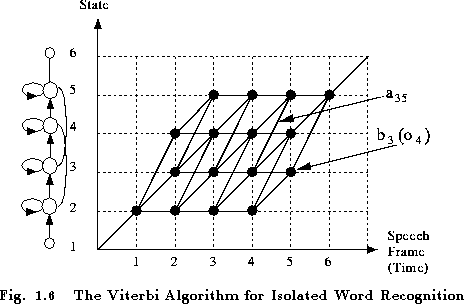
\includegraphics[width=30em]{viterbi_decoding.png}
    \end{center}
    \tiny{\url{http://www.ee.columbia.edu/ln/LabROSA/doc/HTKBook21/node8.html  - viterbi_decoding.gif}}
    % \begin{center}
    %     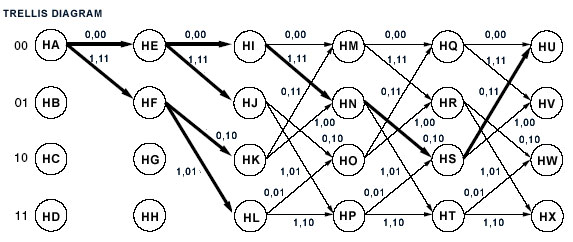
\includegraphics[width=30em]{viterbi_decoding_2.jpg}
    % \end{center}
    % \tiny{http://www.askkia.com/articles/what-is-a-convolutional-encoder-viterbi-algorithm.html - viterbi_decoding_2.jpg}
\end{frame}

\begin{frame}[fragile]\frametitle{Output formats} 

\begin{verbatim}
    0.5 hi how are you
    0.2 hi where are you
    0.1 bey how are you
\end{verbatim}

% Example of 3-best list output with posterior probability for each path. 
% N-best list in Kaldi can be easily extracted from lattices. 
    \begin{center}
        \includegraphics[width=30em]{toy_lattice.ps}
    \end{center}
    % \caption{Word posterior lattice. 
    %     Common parts of hypotheses are effectively represented. 
    %     All outgoing arcs for each node sum to 1.0. }
\end{frame}


\section{Acoustic modelling} %%%%%%%%%%%%%%%%%%%%%%%%%%%%%%%%%%%%%%%%%%%%%%%%%%%%%%%%%%%%%%%%%%

\begin{frame}\frametitle{Acoustic models training} 
    \begin{center}
        % Generated with LaTeXDraw 2.0.5
% Tue Feb 11 11:13:23 CET 2014
% \usepackage[usenames,dvipsnames]{pstricks}
% \usepackage{epsfig}
% \usepackage{pst-grad} % For gradients
% \usepackage{pst-plot} % For axes
\scalebox{1} % Change this value to rescale the drawing.
{
\begin{pspicture}(0,-1.0892187)(7.2534375,1.0892187)
\usefont{T1}{ptm}{m}{n}
\rput(0.44109374,0.40578124){mono}
\usefont{T1}{ptm}{m}{n}
\rput(2.1203125,0.36578125){tri1}
\usefont{T1}{ptm}{m}{n}
\rput(3.68625,0.8857812){tri2a}
\usefont{T1}{ptm}{m}{n}
\rput(3.6567187,-0.17421874){tri2b}
\usefont{T1}{ptm}{m}{n}
\rput(6.1254687,0.50578123){tri2b\_mmi}
\usefont{T1}{ptm}{m}{n}
\rput(6.215469,-0.21421875){tri2b\_bmmi}
\usefont{T1}{ptm}{m}{n}
\rput(6.1534376,-0.8542187){tri2b\_mpe}
\psline[linewidth=0.04cm,arrowsize=0.05291667cm 2.0,arrowlength=1.4,arrowinset=0.4]{->}(1.1071875,0.45578125)(1.7471875,0.43578124)
\psline[linewidth=0.04cm,arrowsize=0.05291667cm 2.0,arrowlength=1.4,arrowinset=0.4]{->}(2.4471874,0.55578125)(3.1871874,0.87578124)
\psline[linewidth=0.04cm,arrowsize=0.05291667cm 2.0,arrowlength=1.4,arrowinset=0.4]{->}(2.4871874,0.41578126)(3.2071874,-0.10421875)
\psline[linewidth=0.04cm,arrowsize=0.05291667cm 2.0,arrowlength=1.4,arrowinset=0.4]{->}(4.1471877,0.03578125)(5.1471877,0.5157812)
\psline[linewidth=0.04cm,arrowsize=0.05291667cm 2.0,arrowlength=1.4,arrowinset=0.4]{->}(4.2671876,-0.20421875)(5.1671877,-0.20421875)
\psline[linewidth=0.04cm,arrowsize=0.05291667cm 2.0,arrowlength=1.4,arrowinset=0.4]{->}(4.1471877,-0.30421874)(5.0871873,-0.82421875)
\end{pspicture} 
}

        \small{\begin{tabular}{lll}
        \hline
        Training method name & Script shortcut \\
        \hline
        Monophone & mono \\
        Triphone  & tri1 \\
        $\Delta + \Delta\Delta$ & tri2a  \\
        LDA+MLLT & tri2b  \\
        LDA+MLLT+MMI & tri2b\_mmi \\
        LDA+MLLT+bMMI & tri2b\_bmmi \\
        MPE & tri2b\_mpe \\
        \hline
        \end{tabular}}
        % \caption{Training partial order among \ac{AM} in our training scripts}
    \end{center}
\end{frame}

\begin{frame}\frametitle{HTK and Kaldi acoustic models} 
    todo copy Kaldi models to the table
    \begin{tabular}{lrr}
        \hline
        \theader{language/method} & \theader{zerogram} & \theader{bigram} \\
        \hline
        \theader{Czech}& & \\
            tri $\Delta+\Delta\Delta$  & 64.5 & 60.4\\
        \hline
        \theader{English}& & \\
           tri $\Delta+\Delta\Delta$  & 50.0 & 17.5 \\
        \hline
    \end{tabular}
    \begin{tabular}{lrr}
        \hline
        \theader{language/method} & \theader{zerogram} & \theader{bigram} \\
        \hline
        \theader{Czech}& & \\
            tri $\Delta+\Delta\Delta$ &   70.7 &   56.6  \\
        \hline
        \theader{English}& & \\
           tri $\Delta+\Delta\Delta$ &   35.7 &   16.2 \\
        \hline
    \end{tabular}
  % \caption{HTK results: Word error rates on test set are obtained by both a~zerogram and a~bigram LM. The~\acp{AM} can be compared with the~basic \term{tri} $\Delta+\Delta\Delta$ Kaldi setup in~Table~\ref{tab:best}.}
\end{frame}

\begin{frame}\frametitle{ASR training results} 
    \begin{tabular}{lrr}
        \theader{language/method}
        & \hphantom{rogram}\llap{\theader{zerogram}} & \theader{bigram} \\
        \hline \\
        \theader{Czech} & & \\
            tri $\Delta+\Delta\Delta$ &   70.7 &   56.6  \\
            tri LDA+MLLT &   68.2 &   53.9 \\
            tri LDA+MLLT+MMI &    65.3  &   49.5 \\
            tri LDA+MLLT+bMMI &    65.3  &   49.3 \\
            tri LDA+MLLT+MPE &    63.8  &   49.2 \\
        \hline \hline \\
        \theader{English} & \\ 
            tri $\Delta+\Delta\Delta$ &   35.7 &   16.2 \\
            tri LDA+MLLT &   33.28 &  15.8 \\
            tri LDA+MLLT+MMI &   25.01 & 10.4  \\
            tri LDA+MLLT+bMMI &   23.9  & 10.2 \\
            tri LDA+MLLT+MPE &   22.41 & 11.1 \\
        \hline
    \end{tabular}
    % \caption{Word error rates for zerogram and bigram LM for different training triphone methods.
    %     The~`tri~$\Delta+\Delta\Delta$' row shows results for a~generative model which is comparable to the~model trained using the~HTK scripts.
    % }
\end{frame}

\begin{frame}\frametitle{Vystadial dataset} 
    \begin{tabular}{lrrr}
        \hline
        dataset & audio[hour] & \# sentences & \# words \\
        \hline
        \textbf{English} & & & \\
                training & 41:30 & 47,463 & 178,110 \\
                development & 01:45 & 2,000 & 7,376 \\
                test & 01:46 & 2,000 & 7,772 \\
        \hline
        \textbf{Czech} & & & \\
                training & 15:25 & 22,567 & 126,333 \\
                development & 01:23 & 2,000 & 11,478 \\
                test & 01:22 & 2,000 & 11,204 \\
        \hline
		\end{tabular}
    % \caption{Size of the~data: length of the~audio (hours:minutes), number of sentences
        % (which is the~same as the~number of recordings), number of words in the~
    % transcriptions.\cite{korvas_2014}}
\end{frame}

\begin{frame}\frametitle{Acoustic model accuracy based training data size} 
    \begin{center}
        \includegraphics[scale=0.7]{images/partial-zerogram.ps}
        % \caption{The~figure displays improving performance of Czech generative AM based on growing size of training data for acoustic modelling. The~zerogram LM allows to evaluate only acoustic modelling, but causes a~high WER. }
    \end{center}
\end{frame}

\begin{frame}\frametitle{Speech recognition accuracy based on LM training data size} 
    \begin{center}
        \includegraphics[scale=0.7]{images/partial-lm-tri2b-bmmi.ps}
        % \caption{Influence of in-domain text size of \ac{LM} on speech recognition quality. The~\ac{AM} \term{tri2b\_bmmi} and parameters are fixed and only \ac{LM} training size varies.}
    \end{center}
\end{frame}


\section{On-line recogniser} %%%%%%%%%%%%%%%%%%%%%%%%%%%%%%%%%%%%%%%%%%%%%%%%%%%%%%%%%%%%%%%%%%

\begin{frame}\frametitle{Components for on-line decoding} 
    \begin{center}
        \psscalebox{1.0 1.0} % Change this value to rescale the drawing.
{
\begin{pspicture}(0,-2.1866903)(14.64,2.1866903)
\rput[bl](6.316553,0.59188676){TODO}
\end{pspicture}
}

    \end{center}
\end{frame}

\begin{frame}\frametitle{(Py)OnlineLatgenRecogniser interface} 
    \begin{itemize}
        \item \term{AudioIn} -- queueing new audio for pre-processing
        \item \term{Decode} -- decoding a~fixed number of audio frames
        \item \term{PruneFinal} -- preparing internal data structures for lattice extraction
        \item \term{GetLattice} -- extracting a~word posterior lattice
        \item \term{GetBestPath} -- extracting a~one best word sequence
        \item \term{Reset} -- preparing the~recogniser for a~new utterance
    \end{itemize}
\end{frame}

\begin{frame}\frametitle{Functional (Py)OnlineLatgenRecogniser demo} 
    \begin{center}
        \lstinputlisting[style=Python]{pykaldi_usage.py}
    \end{center}
\end{frame}


\section[Evaluation in PTI]{Evaluation in Public Transport Information domain}%%%%%%%%%%%%%%%%%%%%%%%%%%%%

\begin{frame}\frametitle{WER, beam, lattice beam} 
    \begin{itemize}
        \item Real Time Factor (RTF) of decoding -- the~ratio of the~recognition time to the~duration of the~audio input,
        \item Latency -- the~delay between utterance end and the~availability of the~recognition results,
        \item Word Error Rate (WER).
    \end{itemize}
\end{frame}

\begin{frame}\frametitle{On-line vs batch decoding} 
    \begin{center}
        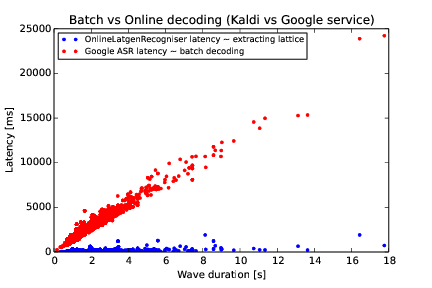
\includegraphics[scale=0.5]{lat_cloud_kaldi.png}
    \end{center}
    % \caption{Almost constant latency of on-line decoder (OnlineLatgenRecogniser) and linearly growing latency of cloud based speech recogniser (Google ASR service) for increasing utterance length.}
\end{frame}

\begin{frame}\frametitle{WER, beam, lattice beam} 
    \includegraphics[scale=0.4]{beam_vs_rtfwer.pdf.ps}
    \includegraphics[scale=0.4]{latbeam_vs_latwer.pdf.ps}
    % \caption{The~upper graph (a) shows that WER decreases with increasing \term{beam} and the~average RTF linearly grows with the~beam.
    %     The~growth of the~95th RTF percentile is limited at 0.6 by setting \term{max-active-states} to 2000, because the~\term{max-active-states} parameters influence presumably the~worst cases with large search space.
    % The~lower graph (b) shows latency growth in response to increasing \term{lattice-beam}.}
\end{frame}

\begin{frame}\frametitle{RTF and Latency} 
    \includegraphics[scale=0.4]{frtf_vs_prc.pdf.ps}
    \includegraphics[scale=0.4]{lat_vs_prc.pdf.ps}
%     \caption{The~percentile graphs show RTF and Latency scores for test data for \term{max-active-sates}=2000, \term{beam}=13, \term{lattice-beam}=5.
% Note that 95 \% of utterances were decoded with the~latency lower that 200ms.}
\end{frame}


\section{Summary} %%%%%%%%%%%%%%%%%%%%%%%%%%%%%%%%%%%%%%%%%%%%%%%%%%%%%%%%%%%%%%%%%%

\begin{frame} \frametitle{Table of content} \tableofcontents \end{frame}

\begin{frame}\frametitle{Achievements} 
    \begin{itemize}
        \item Working real-time on-line speech recogniser
        \item Developed acoustic modeling scripts for Czech and English - accepted to Kaldi svn trunk
        \item Integration of ASR into Alex Dialogue Systems Framework
        \item Improved speech recognition for toll-free line 800 899 998
    \end{itemize}
\end{frame}

\begin{frame}\frametitle{Links and references}
\begin{center}
    {\bf \url{https://github.com/oplatek/kaldi-thesis}}\\
    {\bf \url{https://github.com/UFAL-DSG/pykaldi}}\\
    {\bf \url{https://github.com/UFAL-DSG/alex}}\\
    {\bf \url{http://ufal.mff.cuni.cz/alex-dialogue-systems-framework/}}\\
    {\bf \url{http://www.linkedin.com/in/ondrejplatek}}\\
\end{center}
\end{frame}


\section{Details} %%%%%%%%%%%%%%%%%%%%%%%%%%%%%%%


\begin{frame} \frametitle{Semiring}
\begin{tabular}{lrrrrr}
\hline
Name & $\mathcal{K}$ & $\oplus$ & $ \otimes$ & $\bar{0}$ & $\bar{1}$ \\ 
\hline
Real        & $[0,\infty)$        &  +                     &  * &  0        &  1  \\
Log         & $(-\infty, \infty)$ & $-log(e^{-x} + e^{-y})$ & + &  $\infty$ &  0  \\
Tropical    & $(-\infty, \infty)$ &  min                   &  + &  $\infty$ &  0  \\
\hline
\end{tabular}
% \caption{Semirings used in speech recognition.\cite{openfst_web}}
\end{frame}

\begin{frame} \frametitle{OnlineLatgenRecogniser's lattice}
    TODO insert image of lattice and its one-best path and reference
\end{frame}

\end{document}  % do not remove!
